\documentclass[10pt]{article}
\usepackage[letterpaper]{geometry}
\geometry{verbose,tmargin=1in,bmargin=1in,lmargin=1in,rmargin=1in}
\usepackage{setspace}
\usepackage{ragged2e}
\usepackage{color}
\usepackage{titlesec}
\usepackage{graphicx}
\usepackage{float}
\usepackage{mathtools}
\usepackage{amsmath}
\usepackage[font=small,labelfont=bf,labelsep=period]{caption}
\usepackage[english]{babel}
\usepackage{indentfirst}
\usepackage{array}
\usepackage{makecell}
\usepackage[usenames,dvipsnames]{xcolor}
\usepackage{multirow}
\usepackage{tabularx}
\usepackage{arydshln}
\usepackage{caption}
\usepackage{subcaption}
\usepackage{xfrac}
\usepackage{etoolbox}
\usepackage{cite}
\usepackage{url}
\usepackage{dcolumn}
\usepackage{hyperref}
\usepackage{courier}
\usepackage{url}
\usepackage{esvect}
\usepackage{commath}
\usepackage{verbatim} % for block comments
\usepackage{enumitem}
\usepackage{hyperref} % for clickable table of contents
\usepackage{braket}
\usepackage{titlesec}
\usepackage{booktabs}
\usepackage{gensymb}
\usepackage{longtable}
\usepackage{listings}
\usepackage{cancel}
\usepackage{tcolorbox}
\usepackage[mathscr]{euscript}
\lstset{
    frame=single,
    breaklines=true,
    postbreak=\raisebox{0ex}[0ex][0ex]{\ensuremath{\color{red}\hookrightarrow\space}}
}

% for circled numbers
\usepackage{tikz}
\newcommand*\circled[1]{\tikz[baseline=(char.base)]{
            \node[shape=circle,draw,inner sep=2pt] (char) {#1};}}


\titleclass{\subsubsubsection}{straight}[\subsection]

% define new command for triple sub sections
\newcounter{subsubsubsection}[subsubsection]
\renewcommand\thesubsubsubsection{\thesubsubsection.\arabic{subsubsubsection}}
\renewcommand\theparagraph{\thesubsubsubsection.\arabic{paragraph}} % optional; useful if paragraphs are to be numbered

\titleformat{\subsubsubsection}
  {\normalfont\normalsize\bfseries}{\thesubsubsubsection}{1em}{}
\titlespacing*{\subsubsubsection}
{0pt}{3.25ex plus 1ex minus .2ex}{1.5ex plus .2ex}

\makeatletter
\renewcommand\paragraph{\@startsection{paragraph}{5}{\z@}%
  {3.25ex \@plus1ex \@minus.2ex}%
  {-1em}%
  {\normalfont\normalsize\bfseries}}
\renewcommand\subparagraph{\@startsection{subparagraph}{6}{\parindent}%
  {3.25ex \@plus1ex \@minus .2ex}%
  {-1em}%
  {\normalfont\normalsize\bfseries}}
\def\toclevel@subsubsubsection{4}
\def\toclevel@paragraph{5}
\def\toclevel@paragraph{6}
\def\l@subsubsubsection{\@dottedtocline{4}{7em}{4em}}
\def\l@paragraph{\@dottedtocline{5}{10em}{5em}}
\def\l@subparagraph{\@dottedtocline{6}{14em}{6em}}
\makeatother

\newcommand{\volume}{\mathop{\ooalign{\hfil$V$\hfil\cr\kern0.08em--\hfil\cr}}\nolimits}

\setcounter{secnumdepth}{4}
\setcounter{tocdepth}{4}
\begin{document}

\title{CS 267: HW 1}
\author{April Novak}

\maketitle

\section{Introduction}

The purpose of this assignment is to optimize matrix-matrix multiplication to run as fast as possible on a single processor on the Edison machine at the National Energy Research Scientific Computing Center (NERSC). All methods used for optimizing matrix-matrix multiply pursued here will use \(2n^3\) floating point operations for matrices of size \(n\times n\). Hence, the methods used to optimize matrix-matrix multiplication will focus not on reducing the number of flops, but rather on movement through the memory hierarchy.

\section{Naive Implementation}

This section discusses benchmark results obtained with the naive implementation of matrix-matrix multiply using three nested loops in order to provide the motivation and possible directions to pursue for optimizing matrix-matrix multiplication using a different approach. The {\tt dgemm-naive.c} source file implements matrix-matrix multiplication using a 3-loop structure, where the innermost loop computes the dot product of a row of \(A\) with a column of \(B\), and assigns this to an entry in \(C\). The only attempt at some level of optimization in this code is the encouragement of the compiler in putting the intermediate value {\tt cij} in a register by defining this \textit{technically unnecessary} variable just outside the innermost loop (with iteration counter {\tt k}) such that {\tt cij} is stored in a register for fast operation for all of the {\tt k} loops for a set {\tt i} and {\tt j}.  

\begin{lstlisting}[language=C][H]
void square_dgemm (int n, double* A, double* B, double* C)
{
  for (int i = 0; i < n; ++i)
    for (int j = 0; j < n; ++j)
    {
      double cij = C[i+j*n];
      for(int k = 0; k < n; k++)
        cij += A[i+k*n] * B[k+j*n];
      C[i+j*n] = cij;
    }
}
\end{lstlisting}

This optimization can be demonstrated by changing the above code block to the following, which removes any attempt to encourage the compiler to place {\tt C[i+j*n]} in a register. Although this block has fewer floating point operations, the performance is degraded due to the greater number of slower memory calls. Fig. \ref{fig:1} shows the difference in Mflop/s for (a) the original code that encourages the compiler to place a frequently-used variable in a register and (b) code that removes the technically unnecessary variable {\tt cij} to reduce flops at the expense of more slow memory traffic.

\begin{lstlisting}[language=C][H]
void square_dgemm (int n, double* A, double* B, double* C)
{
  for (int i = 0; i < n; ++i)
    for (int j = 0; j < n; ++j)
    {
      for(int k = 0; k < n; k++)
        C[i+j*n] += A[i+k*n] * B[k+j*n];
    }
}
\end{lstlisting}

\begin{figure}[H]
\centering
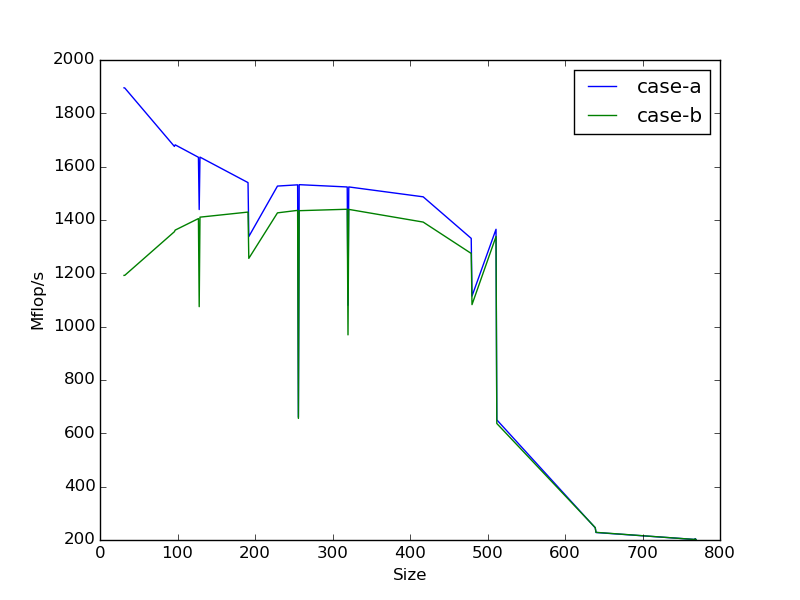
\includegraphics[width=0.6\textwidth]{figures/fig1.png}
\caption{Difference in Mflop/s for (a) the original code encouraging register-allocation for {\tt cij} and (b) the even-more naive code with fewer flops but greater slow memory traffic (no intermediate variable {\tt cij} defined).}
\label{fig:1}
\end{figure}

Encouraging the compiler to place commonly-used variables in the register by defining a variable just outside the loop offers the best improvement in performance speed for smaller matrix sizes. As can be seen from Fig. \ref{fig:1}, for matrices of size greater than about 500\(\times\)500, the improvement is negligible. This may be due to the fact that other processes in the algorithm begin to dominate and bottleneck, rather than the slow memory access of {\tt C[i+j*n]}. However, this technique of encouraging the compiler to place variables in a register is still applicable for the blocked algorithm discussed in the next section, and hence will be investigated as a method for optimization.

Both curves in Fig. \ref{fig:1} show very sharp dips in performance at matrix sizes of 128, 192, 256, 320, and 480, where the speed decreases monotonically after a size of 511. Because these dips in performance occur regardless of if the compiler is being encourage to store values in the register, they are likely due to other features of the memory hierarchy. 

A second way to attempt to optimize the naive algorithm is with the technique of copy optimization, where the layout of one or more matrices is copied to a new location and modified to take advantage of the order in which the data is used. For C, because arrays are stored in column-major layout, the indexing over the rows in \(A\) is expensive. By transposing \(A\), and indexing instead over columns, the code should be able to perform matrix-matrix multiplication faster. Fig. \ref{fig:2} shows the great improvement in the Mflop/s with this simple copy optimization that transposes \(A\) such that it can be accessed in a column-major layout. The improvement is greatest for large matrix sizes, since the extra cost of transposing \(A\) can be amortized by the many more slow memory operations that would be required for larger matrices.

\begin{lstlisting}[language=C][H]
void square_dgemm (int n, double* A, double* B, double* C)
{
  // transpose A so that it is row-major
  double* aij = 0;
  aij = (double*) malloc(n * n * sizeof(double));

  if (aij == NULL)
    printf("Memory allocation error!");

  for (int i = 0; i < n; ++i)
  {
    for (int j = 0; j < n; ++j)
        aij[i + j*n] = A[j + i*n];
  }

  for (int i = 0; i < n; ++i)
    for (int j = 0; j < n; ++j)
    {
      double cij = C[i+j*n];
      for( int k = 0; k < n; k++ )
        cij += aij[k+i*n] * B[k+j*n];
      C[i+j*n] = cij;
    }
  free(aij);
}
\end{lstlisting}

\begin{figure}[H]
\centering
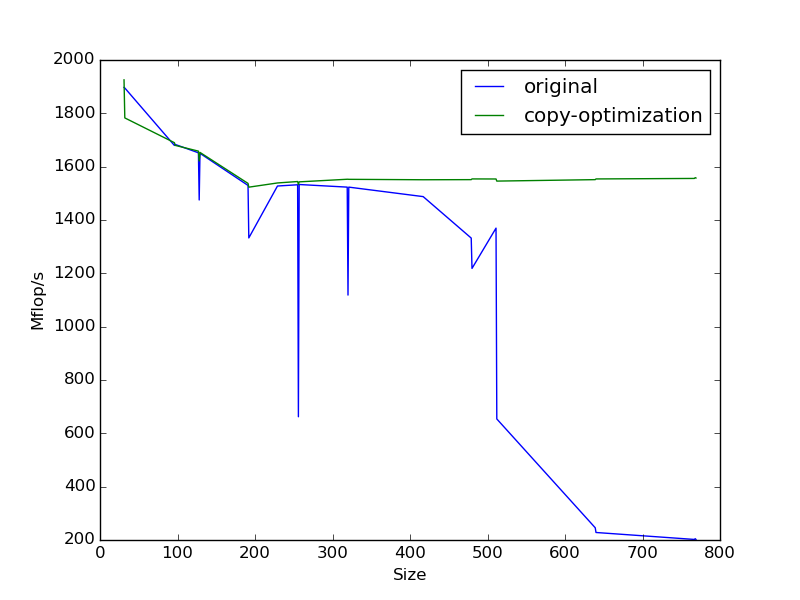
\includegraphics[width=0.6\textwidth]{figures/copy-optimization.png}
\caption{Difference in Mflop/s for (a) the original code and (b) the copy-optimization code that transposes \(A\) so that it can be accessed in a column-major layout.}
\label{fig:2}
\end{figure}

\section{Blocked Implementation}

\section{Cori Intel Xeon Phi Optimization}

\end{document}

